\include{MeijeCours}

\newboolean{versionprof}  % Cette variable booléenne permet le contrôle de la compilation selon la version professeur (avec les preuves, commentaires pédagogiques etc...) si true ou selon la version élève (de ''base'') si false.
\setboolean{versionprof}{false}

% =============================================================================================
%                                                                                      Début du texte 
% =============================================================================================

\author{Spé NSI - Lycée du parc}  % Pour spécifier l'auteur qui sera affiché sous le titre
\title{TD : Algorithme des K plus proches voisins}  % Titre 
\date{Année 2020-2021} %en utilisant \today on obtiendra la date courante lors de la production du document
\renewcommand{\thesection}{\Roman{section}}  % permet de numéroter les sections en chiffres romains
\pagestyle{fancy}

\lhead{NSI}   %  Indiquer la classe ici  
\rhead{Algorithme des K plus proches voisins}		% Indiquer la date pour rendre le devoir ici


\fancyfoot[C]{\thepage} % bas de page : centre par exemple:  - \thepage\ -
\fancyfoot[L]{} % bas de page : gauche
\fancyfoot[R]{} % bas de page : droite
\newcommand{\p}[1]{ \left( #1 \right)}   %parenthèse
\newcommand\abs[1]{|{#1}|}

\begin{document}

\maketitle  %produit le titre conformément aux instructions données par \author, \date ...etc
\thispagestyle{empty}
% ------------------------------------------------   Introduction   -------------------------------------------
\vskip 1cm
\renewcommand{\abstractname}{Introduction\hfill}
\begin{abstract} 

On se propose ici d'écrire un algorithme dérivé de l'algorithme de tri par insertion dont le but est d'obtenir les k plus petits éléments d'une liste. On verra ensuite comment adapter et utiliser cet algorithme pour résoudre un problème de classification.
\end{abstract} 


\section{Les k plus petits éléments d'une liste}

\noindent{\bf Question 1}
\medskip

Compléter la fonction suivante après avoir bien lu sa spécification dans la docstring.

Si vous n'y arrivez pas, vous pouvez ouvrir votre cours au chapitre qui traite des tris et consulter le paragraphe sur le tri par insertion.
\begin{lstlisting}[escapeinside =;;]
def insertion_croissante(L, x):
    """
    L est une liste de flottants qui est tri;\it é;e par ordre croissant 
    et x est un flottant.
    Ajoute l';\it é;l;\it é;ment x ;à; la liste L en l'ins;\it é;rant ;à; sa place.
    """
    

\end{lstlisting}
\lignes{10}


\noindent{\bf Question 2}
\medskip

Pour déterminer les k plus petits éléments de la liste L, on procède en deux temps :

    On range un à un les k premiers éléments de L dans une nouvelle liste \verb+plus_petits+

(ce qui revient à faire un tri par insertion de cette partie de L).

On parcourt le reste de la liste et pour chaque élément x, on le compare avec le plus grand de la liste \verb+plus_petits+.
Si x est plus petit, on retire le dernier élément de \verb+plus_petits+ et on y insère x à l'aide de \verb+insertion_croissante+.


Compléter le code de la fonction suivante en conséquence.

\begin{lstlisting}[escapeinside =;;]
def k_plus_petits(L, k):
    """
    Renvoie la liste des k plus petits ;é;l;é;ments de L
    """
    
    assert type(k) == int and k > 0, "k doit ;ê;tre un entier > 0"
    assert k <= len(L), "La liste ne contient pas assez d';é;l;é;ments"
    
    
    plus_petits = []
    
    #  Partie ;à; compl;é;ter
    #  Indication : il y a deux boucles ;à; ;é;crire

    return plus_petits
    
\end{lstlisting}
\lignes{16}



\section{Les k plus proches voisins}

L'algorithme des k plus proches voisins est essentiellement le même que celui qu'on vient d'écrire. Son intérêt réside dans son utilisation pour classifier des données en se basant sur la connaissance des classes pour un grand nombre d'autres données de même type. En cela il se range dans la famille des algorithmes d’apprentissage automatique (machine learning).

Examinons un exemple : Un botaniste a mesuré quatre éléments caractéristiques de 150 fleurs d'Iris dont 50 de chacune de trois espèces différentes (ce sont les classes qui nous intéressent ici). Il a ainsi obtenu un ensemble de 150 enregistrements comportant pour chaque fleur :
\begin{itemize}

   \item   la longueur des sépales (en cm)
  \item     la largeur des sépales (en cm)
    \item   la longueur des pétales (en cm)
    \item   la largeur des pétales (en cm)
    \item   l’espèce d’iris : Iris setosa, Iris virginica ou Iris versicolor
\end{itemize} 
\medskip

On ne peut pas représenter simmultanément quatre données numériques dans le plan mais, si on se restreint par exemple à la longueur des pétales en abscisse et la largeur en ordonnée, on obtiendrait l'ensemble des points suivants :


\begin{center}
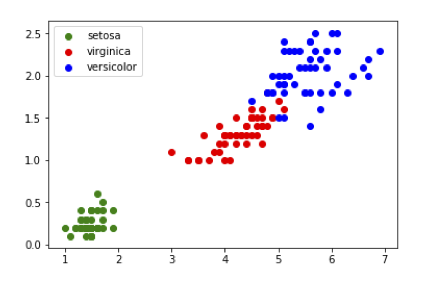
\includegraphics[width=10 cm]{Iris_sepales.png}
\end{center}

Les données sont incluses dans le fichier présent sur le réseau : C'est la définition de la liste  \verb+BDIris+

(base de données) comportant 150 éléments qui sont des tuples de 5 éléments sous la forme :

\verb+(long_sep, larg_sep, long_pet, larg_pet, esp)+

où les quatre premiers éléments sont des flottants qui correspondent aux mesures et le cinquième est un entier entre 0 et 2 qui code l'espèce (0 pour Iris setosa, 1 pour Iris virginica et 2 pour Iris versicolor)

On va utiliser ces données pour essayer de déterminer à quelle espèce appartient une fleur connaissant les quatre mesures (longueur et largeur des sépales et pétales). On considère une fleur dont on a les mesures mais pas l'espèce (code -1 pour l'espèce):

\verb+nouv_fleur = (long_sep, larg_sep, long_pet, larg_pet, -1)+
\bigskip

\noindent{\bf Question 3}
\medskip

Pour mesurer à quel point cette fleur ressemble à chacune des 150 de la base de données, on va utiliser une distance. Parmi les k plus proches de cette fleurs (c'est à dire les k plus petites distances à \verb+nouv_fleur+), on va ensuite déterminer quelle est l'espèce la plus fréquente. La fonction suivante calcule la distance entre deux fleurs. 

Compléter la fonction suivante qui calcule la distance entre deux fleurs. n utilisera la distance euclidienne : \begin{center}
$\sqrt{(x_{2}-x_{1})^{2}+(y_{2}-y_{1})^{2}+(z_{2}-z_{1})^{2}+(t_{2}-t_{1})^{2}}$
\end{center}

\begin{lstlisting}[escapeinside =;;]
from math import sqrt
def distance(fleur_1, fleur_2):
    """Renvoie la distance entre les deux fleurs."""
    
    
    
    
; ;
\end{lstlisting}



\noindent{\bf Question 4}
\medskip

Adapter la fonction \verb+insertion_croissante+  pour en déduire la fonction \verb+insertion_fleur+ en utilisant la fonction \verb+distance+ pour comparer les distances de deux fleurs avec \verb+nouv_fleur+. 

\begin{lstlisting}[escapeinside =;;]
def insertion_fleur(nouv_fleur, L, fleur):
    """
    nouv_fleur est la fleur de r;é;f;é;rence. L est une liste de fleurs 
    qui est tri;é;e par ordre croissant des distances ;à; nouv_fleur.
    Ajoute fleur ;à; la liste L en l'ins;é;rant ;à; sa place pour la 
    distance ;à; nouv_fleur.
    """
    
    ; ; 
    \end{lstlisting}
    
\lignes{12}

\noindent{\bf Question 5}
\medskip

Adapter la fonction \verb+k_plus_petits+ pour en déduire la fonction \verb+k_NN+ (de l'anglais k-nearest neighbors) à l'aide de la fonction \verb+insertion_fleur+. On utilisera la liste \verb+BDIris+ comme une variable globale.

\begin{lstlisting}[escapeinside =;;]
def k_NN(nouv_fleur, k):
    """
    Renvoie la liste de k fleurs les plus proches de nouv_fleur.
    """
    
    assert type(k) == int and 1 <= k <= 150, 
    "k n'est pas entier entre 1 et 150"
    
    plus_proches = []
    
    #
    #  Partie ;à; compl;é;ter
    #
    
    return plus_proches    
    ; ; 
    \end{lstlisting}
\eject
\lignes{15}

\noindent{\bf Question 6}
\medskip

Lire et compléter les codes des fonctions pour en déduire une fonction qui renvoie le code de l'espèce que la méthode des k plus proches voisins attribue à \verb+nouv_fleur+.

\begin{lstlisting}[escapeinside =;;]
def indice_max(L):
    """
    L est une liste non vide d'entiers. Renvoie l'indice de la 
    premi;è;re occurence du maximum de la liste.
    """
    
    #
    #  Partie ;à; compl;é;ter. 
    #
    
    
def prediction_espece(nouv_fleur, k):
    """
    Renvoie le code de l'esp;è;ce que la m;é;thode des k plus proches 
    voisins attribue ;à; nouv_fleur d'apr;è;s les donn;é;es de BDIris. 
    Dans le cas d';é;galit;é;, n'importe laquelle des r;é;ponses possibles 
    est bonne.
    """
    
    plus_proches = k_NN(nouv_fleur, k)
    compteurs = [0,0,0]  # compteurs[i] va compter les 
    # fleurs d'esp;è;ce cod;é;e par i.

    #
    #  Partie ;à; compl;é;ter. 
    #


    return indice_max(compteurs)
\end{lstlisting}

\eject

\lignes{30}
\end{document}




